
\section{ Закон Хаббла. Расстояния в космологии.}

Вселенная расширяется. Точного описания этого эффекта нет, но существуют различные модели(типа \href{https://en.wikipedia.org/wiki/Lambda-CDM_model}{$\Lambda$CDM}, о которой также пойдет речь) описания этого.

В данном билете рассказывается о сути закона Хаббла, о вышеупомянутой модели, о различных расстояниях, использумых при описании(потому что в расширяющейся вселенной может быть удобно говорить о разных расстояниях).

\subsection{Расстояния в космологии}

Если представить себе, что всеселнная не расширяется, а объекты не имеют пекулярных скоростей(то есть абсолютно всё покоится), то именно в такой системе мы можем говорить о \textbf{сопутствующих расстояниях(comoving distance)} - расстояниях в системе отсчета, когда мы зафиксировали все галактики в какой-то момент времени(это важно - фиксируют его для текущего времени). Обозначать его я буду буквой $\chi$.

\textbf{Собственное расстояние(proper distance)} определяется через масштабный фактор a:

\begin{equation}
d = a \cdot \chi
\label{eq:18_proper}
\end{equation}

Наблюдая свет, приходящей от галактики, мы можем измерять \textbf{красное смещение} z, смотря на особые спектральные линии(например линия 21 см или линия HI). Красным оно называется, потому что длина волны увеличивается, тем самым смещая спектр в сторону длинноволнового. Определение и связь смещения с масштабным фактором показаны на рисунке \ref{fig:18_redshift}.

\begin{figure}[H]
	\centering
	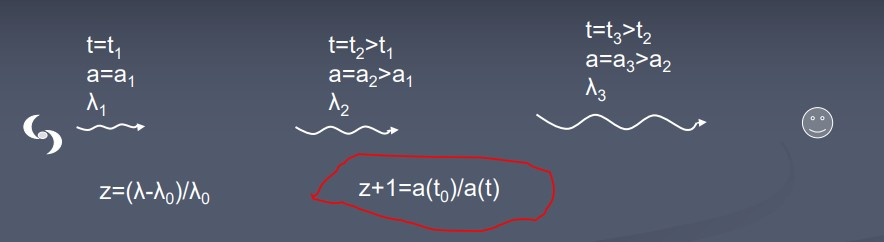
\includegraphics[width=0.7\linewidth]{18_redshift}
	\caption{Красное смещение}
	\label{fig:18_redshift}
\end{figure}

Есть так называемое \textbf{фотометрическое расстояние} - оно определяется из формулы для потока:

\begin{equation}
f = \frac{L}{4 \pi d_{ph}^2}
\label{eq:18_photometric}
\end{equation}

Таким образом, оно просто связывается с собственным расстоянием, умножая его на (1+z), потому что именно во столько(из определения) уменьшается энергия фотонов:

\begin{equation}
d_{ph} = \frac{a(t_0)}{a(t_{em})} \cdot d = \frac{a^2(t_0)}{a(t_{em})} \chi
\label{eq:18_photo_proper}
\end{equation}

Существует еще одно важное расстояние - \textbf{Угловое(угломерное) расстояние}. Зная размер галактики s, зная угол под которым мы видим галактику, мы можем использовать классическую формулу для определения расстояния:

\begin{equation}
d_{\theta} = \frac{s}{tg(\alpha)}
\label{eq:18_angular}
\end{equation}

По предположению, вселенная плоская(в том смысле, что у нее нет кривизны), и потому угол между фотонами сохраняется во времени. Однако галактика могла испустить фотон, который мы детектируем, в разные моменты вселенной(так как вселенная эволюционирует, меняется количественное соотношение типов вещества, скорость расширения не остаётся постоянной), поэтому красное смещение не однозначно показывает это расстояние. Из рисунка \ref{fig:18_angular}(слайд с лекции), для галактик с одинаковым s в разные моменты времени z может быть разным(но собственное расстояние будет одинаковым на момент испускания):

\begin{figure}[H]
	\centering
	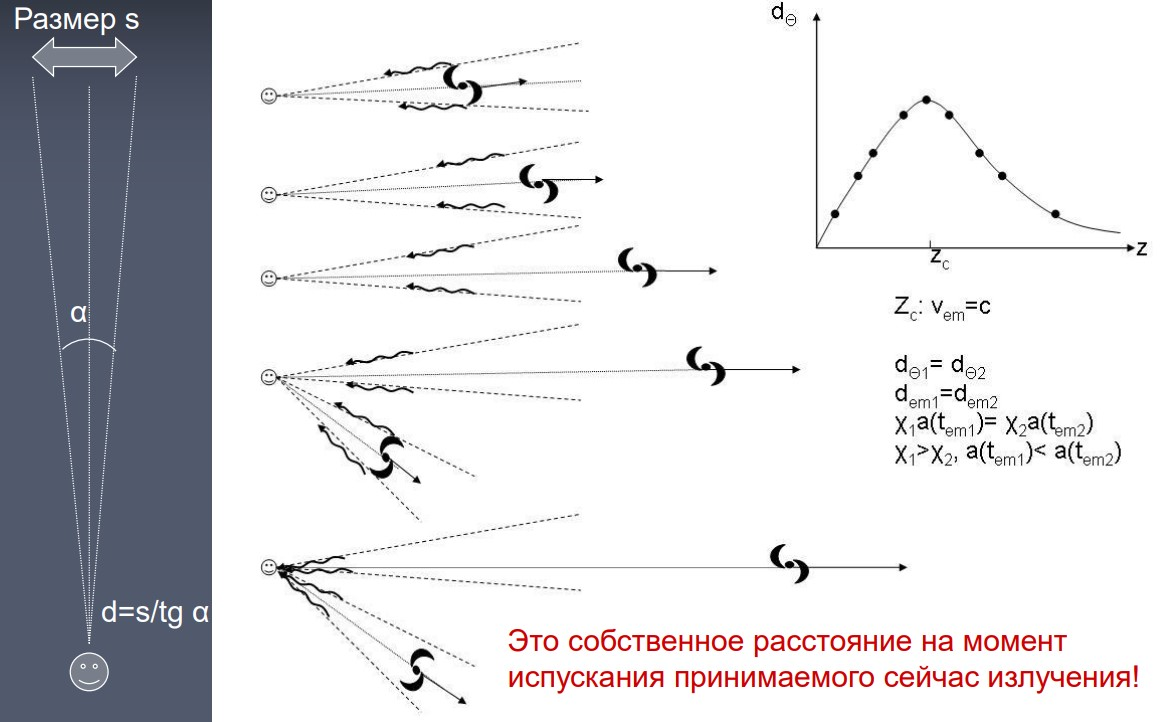
\includegraphics[width=0.7\linewidth]{18_angular}
	\caption{Угловое(углометрическое) расстояние}
	\label{fig:18_angular}
\end{figure}

Мы ввели все основные расстояния, которые и будем связывать друг с другом, но есть еще одно - время путешествия(жизни) фотона. Оно лежит где-то между собственным расстоянием в момент испускания фотона, и собственным расстоянием в настоящий момент.

\begin{equation}
d_l = c \cdot \Delta t
\label{eq:18_lifetime}
\end{equation}

Связь всех этих величин такая($d_{pm}$ - собственное расстояние в настоящий момент, $t_{em}$ - момент испускания фотона):

\begin{equation}
d_{\theta} = a(t_{em}) \chi = \frac{d_{pm}}{1+z} = \frac{d_{ph}}{(1+z)^2}
\label{eq:18_link}
\end{equation}

При этом расстояние $d_{pm} = d$ можно вычислить через постоянную Хаббла(о ней следующий пункт), красное смещение и скорость света:

\begin{equation}
d = \frac{c}{(1-\alpha)H_0} [(1 + z)^{1-\alpha} - 1]
\label{eq:18_distance_h}
\end{equation}

\subsection{Закон Хаббла}

Закон Хаббла в классическом определении - связь скорости удаления галактик в зависимости от собственного расстояния между ними. $H_0$ - коэффициент пропорциональности, называемый постоянной Хаббла(которая на самом деле не постоянна, но берется значение в текущий момент времени).

\begin{equation}
v = H_0 r
\label{eq:18_classic_hubble}
\end{equation}

Сформулировать закон можно также и через масштабный фактор:

\begin{equation}
v = \dot{d}, d = a(t) \chi; \implies v = H d,  H = \frac{\dot{a}(t)}{a(t)}
\label{eq:18_hubble_law}
\end{equation}

Это был вывод в предположении, что галактики не имеют пекулярных скоростей(иначе сама $\chi$ не будет const).

Опуская то, откуда мы это знаем(нам дал \href{https://en.wikipedia.org/wiki/Friedmann_equations}{Бог}), масштабный фактор имеет степенную зависимость от времени, и степень разная для разных типов среды, доминирующих во вселенной:

\begin{equation}
a(t) \sim t^{\frac{1}{\alpha}}, \text{Пыль(материя), $\alpha=1.5$; Излучение, $\alpha=2$; Косм.пост.(темная энергия), $\alpha=0$}
\label{eq:18_scale_factor}
\end{equation}

Тогда из \ref{eq:18_scale_factor} и \ref{fig:18_redshift} следует:

\begin{equation}
H = H_0 (1 + z)^{\alpha}
\label{eq:18_hubble_z}
\end{equation}

Тогда, мы можем найти выражение для сопутствующего расстояния(а через него - и для всех остальных):

\begin{multline}
\text{Для света, } 0 = ds^2 = c^2dt^2 - a^2(t)dl^2 \implies \chi = \int dl = \bigg\{ \text{хитро меняя $\frac{dt}{a(t)}$} \\ \text{на $\frac{dz}{a(t_0) H(z)}$} \bigg\} = \frac{c}{a(t_0)} \int_{0}^{z} \frac{dz}{H(z)} = \frac{c}{a(t_0)H_0} \frac{1}{1-\alpha}[(1+z)^{1-\alpha} - 1]
\label{eq:18_distances}
\end{multline}

Отсюда легко получить, почему для близких галактик всё 'по Допплеру':

\begin{equation}
z \ll 1, d = \frac{c z}{H_0}, \text{при этом } d \cdot H_0 = v \implies v = c z, v \sim z
\label{eq:18_semidoppler}
\end{equation}

Когда присутствует несколько типов сред, то выражение для H следующее:
%\href{https://en.wikipedia.org/wiki/Lambda-CDM_model}{$\Lambda$CDM}

\begin{equation}
H^2(z) = H_0^2[\Omega_{radiation}(1+z)^{4} + \Omega_{matter}(1+z)^{3} + \Omega_{curvature}(1+z)^{2} + \Omega_{\Lambda}]
\label{eq:18_hubble_const}
\end{equation}

Где каждое слагаемое в скобках отвечает за свой тип среды: 1 - излучение, 2 - материя, 3 - кривизна(о которой речи не было, по предположению плоскости вселенной), 4 - темная энергия(вакуум, космическая постоянная, 'стоимость существования пространства'), а $\Omega$ - относительное содержание типа среды во вселенной(значение от 0 до 1, $\sum \Omega_i = 1$)

В вышеупомянутой \href{https://en.wikipedia.org/wiki/Lambda-CDM_model}{$\Lambda$CDM} модели, в простой реализации оставляют только 2 и 4 слагаемые, кладя соответствующие $\Omega$ равными ~0.3 и ~0.7 соответственно.
